\documentclass[10pt,twocolumn]{article}
\usepackage[a4paper]{geometry}
\usepackage{placeins}
\usepackage[font=small,skip=0pt]{caption}
\usepackage{times}
\usepackage{graphicx}
\usepackage{amssymb}
\usepackage{url,hyperref}
\usepackage{enumitem}

\hypersetup
{
    pdfauthor={lambdaShade, dolu1990},
    pdfsubject={Short presentation},
    pdftitle={SpinalHDL : A comprehensive HDL language}
}

\newgeometry{left=2.5cm,right=2.5cm,top=1.0cm,bottom=2cm}

\setlength\parindent{0pt}

\begin{document}
	
	\title{\textbf{\textsc{SpinalHDL} : A comprehensive HDL language}}
	
	\author{dolu1990, lambdaShade\\}
	
	\maketitle
	\thispagestyle{empty}
	
	\begin{abstract}
		\textsc{SpinalHDL} is a new HDL language offering the ability to break the limitations of the most common hardware description languages, like \textit{VHDL} and \textit{Verilog}.
	\end{abstract}

	\section{\textsc{SpinalHDL} Structure}
		\textsc{SpinalHDL} is a library constructed over the Scala internal DSL, allowing the user to design productively his digital hardware. The user designs can be converted to \textit{VHDL} files for synthesis with any PLD/FPGA/ASIC specialized toolchain. 
		\begin{figure}[!h]
		  \begin{center}
		    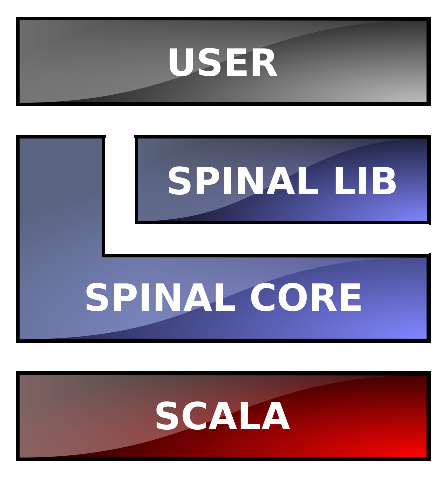
\includegraphics[width=4.5cm]{graphics/spinalstructure.eps}
		  \end{center}	
		  \caption{\textsc{SpinalHDL} structure layers}
		  \label{fig:spinalstructure}
		\end{figure}
		\FloatBarrier
		The Spinal library is separated in two parts : one - the \textbf{core} - providing basic elements for hardware description and another one on it - the \textbf{lib} - providing interfaces and utilities for construct powerful design and help the user in his tasks.
		
	\section{Highlights}
		Here's a list of the main advantages of \textsc{SpinalHDL} comparatively to \textit{VHDL} and \textit{Verilog} :
		\begin{itemize}[itemsep=0ex,label=$\textendash$]
			\item No restriction with the genericity of your hardware description by using the power of the Scala language.
			\item No more endless wiring : create and connect complex buses like \textit{AXI} in only one text line.
			\item Evolving capabilities : create your own buses definitions and abstraction layers.
			\item Reduce code size by a high factor - especially for wiring - allowing you to have a better visibility, more productivity and fewer headaches.
			\item Available user friendly IDE with auto-completion, error highlight, navigation shortcut and many others.
			\item Extract information from your digital design and generate files containing data about some latency and addresses, for example.
			\item Bidirectional translation between bunch of bits and any data type/structures. Useful to load a complex data structure from a CPU interface.
			\item Check for combinational loop/latch presence.
			\item Check for user unintentional cross clock domain violations.
		\end{itemize}
	
	\section{Core primitives}
		\begin{itemize}[itemsep=0ex,label=$\textendash$]
			\item \textbf{Base Types} ~ Bool, Bits, UInt, SInt, Enumeration.
			\item \textbf{Bundle} ~ Allows to describe a data structure with the possibility to specify the direction (in, out) for each element. Useful to describe buses.
			\item \textbf{Reg} ~ Creates a register signal.
			\item \textbf{Vec} ~ Allows to create an array of data.
			\item \textbf{Mem} ~ Gives the possibility to manipulate memory.
			\item \textbf{BlackBox} ~ Allows to instantiate a third party HDL component.
		\end{itemize}
	
	\section{Lib primitives}
		\begin{itemize}[itemsep=0ex,label=$\textendash$]
			\item \textbf{Interfaces} ~ Flow, handshake, fragments, ...
			\item \textbf{Components} ~ FIFOs, inter-clock domain bridges, ...
			\item \textbf{Peripherals} ~ UART, ...
			\item \textbf{Utils} ~ Gray conversions, counters, one-hot encoding, majority vote...
			\item \textbf{Digital design analysis} ~ Tool for pipeline latency evaluation.
		\end{itemize}
		
	\section{To go further...}
		\begin{itemize}[itemsep=0ex,label=$\textendash$]
			\item Repositories available on Github : \\ \begin{footnotesize} \url{https://github.com/SpinalHDL} \end{footnotesize}
			\item Some examples : \\ \begin{footnotesize} \url{https://github.com/SpinalHDL/SpinalHDL/blob/master/README.md} \end{footnotesize}
		\end{itemize}
		
	%\bibliographystyle{abbrv}
	%\bibliography{bib}
\end{document}
